\subsection{Version control system}

\subsubsection{Apache Subversion}

Apache Subversion (often abbreviated SVN, after the command name svn) is a software versioning and a revision control system distributed under a free license. Developers use Subversion to maintain current and historical versions of files such as source code, web pages, and documentation. Its goal is to be a mostly-compatible successor to the widely used Concurrent Versions System (CVS).\newline

The open source community has used Subversion widely: for example in projects such as Apache Software Foundation, Free Pascal, FreeBSD, GCC, Django, Ruby, Mono, SourceForge, PHP and MediaWiki. Google Code also provides Subversion hosting for their open source projects. BountySource systems use it exclusively. CodePlex offers access to Subversion as well as to other types of clients.\newline

The corporate world has also started to adopt Subversion. A 2007 report by Forrester Research recognized Subversion as the sole leader in the Standalone Software Configuration Management (SCM) category and as a strong performer in the Software Configuration and Change Management (SCCM) category.\newline

Subversion was created by CollabNet Inc in 2000 and is now a top-level Apache project being built and used by a global community of contributors.

\subsubsection{GitHub}

GitHub is a web-based hosting service for software development projects that use the Git revision control system. GitHub offers both commercial plans and free accounts for open source projects.\newline

Collaboration on Github is not complicated but also not intuitively clear for beginners because not all parts of the workflow are incorporated into the Github user interface. This description describes the structure of collaboration between the contributors and the maintainers of a project that is hosted on github. For every step in the workflow the respective git commands are given for reference.\newline

\begin{figure}[htb]
	\centering
	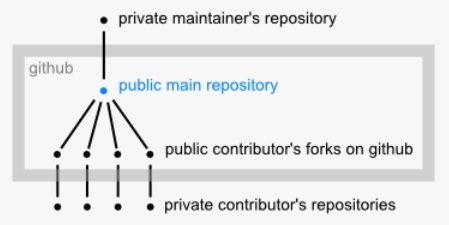
\includegraphics[width=0.6\textwidth]{prestudy/github.jpg}
	\caption{Distributed setup of git repositories\cite{git:repositories}}
	\label{fig:github}
\end{figure}

\newpage
